%%%%%%%%%%%%%%%%%%%%%%%%%%%%%%%%%%%%%%%%%
% a0poster Portrait Poster
% LaTeX Template
% Version 1.0 (22/06/13)
%
% The a0poster class was created by:
% Gerlinde Kettl and Matthias Weiser (tex@kettl.de)
%
% This template has been downloaded from:
% http://www.LaTeXTemplates.com
%
% License:
% CC BY-NC-SA 3.0 (http://creativecommons.org/licenses/by-nc-sa/3.0/)
%
%%%%%%%%%%%%%%%%%%%%%%%%%%%%%%%%%%%%%%%%%

%----------------------------------------------------------------------------------------
%	PACKAGES AND OTHER DOCUMENT CONFIGURATIONS
%----------------------------------------------------------------------------------------

\documentclass[a0,portrait]{a0poster}

\usepackage{multicol} % This is so we can have multiple columns of text side-by-side
\columnsep=100pt % This is the amount of white space between the columns in the poster
\columnseprule=3pt % This is the thickness of the black line between the columns in the poster

\usepackage[svgnames]{xcolor} % Specify colors by their 'svgnames', for a full list of all colors available see here: http://www.latextemplates.com/svgnames-colors

%\usepackage{times} % Use the times font
\usepackage{palatino} % Uncomment to use the Palatino font
\usepackage[utf8]{inputenc}
\usepackage{textcomp}
\usepackage{minted}
\usepackage[french]{babel}
\usepackage{graphicx} % Required for including images
\graphicspath{{figures/}} % Location of the graphics files
\usepackage{booktabs} % Top and bottom rules for table
\usepackage[export]{adjustbox}
\usepackage{hyperref}
\usepackage[style=authoryear]{biblatex}
\usepackage[font=small,labelfont=bf]{caption} % Required for specifying captions to tables and figures
\usepackage{amsfonts, amsmath, amsthm, amssymb} % For math fonts, symbols and environments
\usepackage{wrapfig} % Allows wrapping text around tables and figures

\addbibresource{extracted.bib}

\begin{document}

%----------------------------------------------------------------------------------------
%	POSTER HEADER
%----------------------------------------------------------------------------------------

% The header is divided into two boxes:
% The first is 75% wide and houses the title, subtitle, names, university/organization and contact information
% The second is 25% wide and houses a logo for your university/organization or a photo of you
% The widths of these boxes can be easily edited to accommodate your content as you see fit

\begin{minipage}[b]{0.5\linewidth}
\veryHuge \color{NavyBlue} \textbf{Optimisation d'échangeurs de chaleur à films ruisselants} \color{Black}\\ % Title
\large \textit{\url{https://github.com/celliern/arc_2017}}\\[2cm] % Subtitle

\huge \textbf{Nicolas CELLIER}\\[0.5cm] % Author(s)
\huge Laboratoire LOCIE\\
Campus Universitaire Savoie Technolac\\
73376 Le Bourget du Lac\\[0.4cm] % University/organization
\Large \texttt{contact@nicolas-cellier.net} --- +336 71 37 74 67\\
\end{minipage}
%
\begin{minipage}[b]{0.5\linewidth}
\begin{flushright}
	
\includegraphics[height=5cm]{logo-arc-72dpi}
    \hspace{1cm}
    
\includegraphics[height=5cm]{logo-ara}
	\hspace{1cm}
	
\includegraphics[height=5cm]{locie-logo}
\end{flushright}
\vspace{10cm}
\end{minipage}

\vspace{1cm}

\color{DarkSlateGray}

\begin{multicols}{2}
    \setlength{\columnseprule}{0pt}

    \section*{Introduction}

    Phénomène observable dans les rues durant une averse particulièrement intense, le film ruisselant est un écoulement complexe qui trouve des applications au sein du génie des procédés industriels.

    Échangeurs de chaleur, évaporateurs sont des équipements technologiques pouvant tirer profit des caractéristiques particulières de ce phénomène.

    En s'écoulant sur une surface plane et sous certaines conditions hydrodynamiques, un fluide pourra commencer à se déstabiliser et présenter des séries d'ondelettes à sa surface. Ce phénomène s'accompagne d'une forte intensification des transferts (thermiques et matière).

    \begin{multicols}{2}
        \begin{center}\vspace{.2cm}
            \adjincludegraphics[height=8cm,width=.95\columnwidth,trim={0 {.7\height} 0 0},clip]{street_flow_01}
            \captionof{figure}{Film d'eau ruisselant le long d'une rue en pente}
        \end{center}\vspace{.2cm}
        \columnbreak
        \begin{center}\vspace{.5cm}
            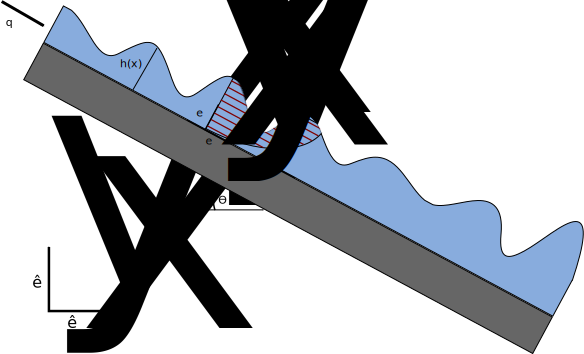
\includegraphics[height=8cm]{thinfilm_unstable}
        	\captionof{figure}{Schéma d'un film ruisselant instable}
        \end{center}\vspace{.5cm}
    \end{multicols}

    \columnbreak

    \section*{Problématique}
    \begin{itemize}
    	\item[$\bullet$] Couplage entre l'hydrodynamique et les phénomènes de transfert relativement peu étudié.
    	\item[$\bullet$] Sa maîtrise peut mener à une intensification des phénomènes au cœur d'équipements technologiques et à la réduction de leur encombrement.
    	\item[$\bullet$] Nécessité de modéliser correctement l'hydrodynamique du film, et le couplage avec les transferts de chaleurs / de masse.
    \end{itemize}

    \subsection*{Les modèles}
    \begin{itemize}
	    \item[$\bullet$] Modèles industriels nombreux, mais imparfaits [\cite{Killion2001}].
    	\begin{itemize}
    		\item Beaucoup de corrélations basés sur films plats.
    		\item Les films ruisselants verticaux sont instables quelque soit le Reynolds [\textcite{Miller1998a}].
    		\item Incompréhension des interactions hydro / thermique menant à l'intensification de transfert
    	\end{itemize}
	    \item[$\bullet$] Simulation numérique direct, couteuse
    	\begin{itemize}
    		\item Basé sur la résolution directe des équations de Navier et Stokes et de Fourrier.
    		\item Le coût calcul interdit un travail d'optimisation en des temps raisonnables.
    	\end{itemize}
        \color{DarkRed}{
	    \item[$\bullet$] Modèles asymptotiques (méthode retenue)
    	\begin{itemize}
    		\item Basé un développement en couche limite adapté aux films ruisselants
    		\item Limité à un domaine de paramètres restreints (faible Reynolds et Peclet).
    		\item Travail important sur les équations en amont.
    	\end{itemize}
        }
    \end{itemize}
\end{multicols}

\begin{center}
    \line(1,0){1800}
\end{center}

\section*{Travaux engagés}
\subsection*{Écriture d'un solveur différence fini 1D axé prototypage \url{https://locie.github.io/triflow/}}
    L'ensemble des simulations ont été effectué par un solveur écrit dans le cadre de la thèse, publié sous license open-source. Par la prise en compte de la structure creuse et l'utilisation de framework de compilation haute performance (via la librarie Theano), l'utilisation d'algorithmes spécialisé et de schéma temporels implicite d'ordres élevés, ce solveur permet d'écrire et de tester rapidement nos modèles.

\begin{multicols}{2}
    \subsection*{Modélisation hydrodynamique}
    Modèle asymptotique intégré sur la hauteur du film a été développé, basé sur les travaux de \textcite{Ruyer-Quil2000}.

    \begin{multicols}{2}
        \begin{align*}
            \partial_t h =& -\partial_x q\\
            3 \mathrm{Re} \partial_t q =& \frac{5}{6} h
                \left(
                    1 - Ct \partial_x h + We \partial_{x,x,x} h
                \right)\\
            & - \frac{5}{2}\frac{q}{h^2}
            - \frac{5}{4} M \partial_x \theta \\
            & + 3 \mathrm{Re}
                \left(
                    \frac{9}{7}\frac{q}{h}^2 \partial_x h - \frac{17}{7}\frac{q}{h} \partial_x q
                \right)
        \end{align*}
        \columnbreak
        \begin{center}\vspace{.5cm}
            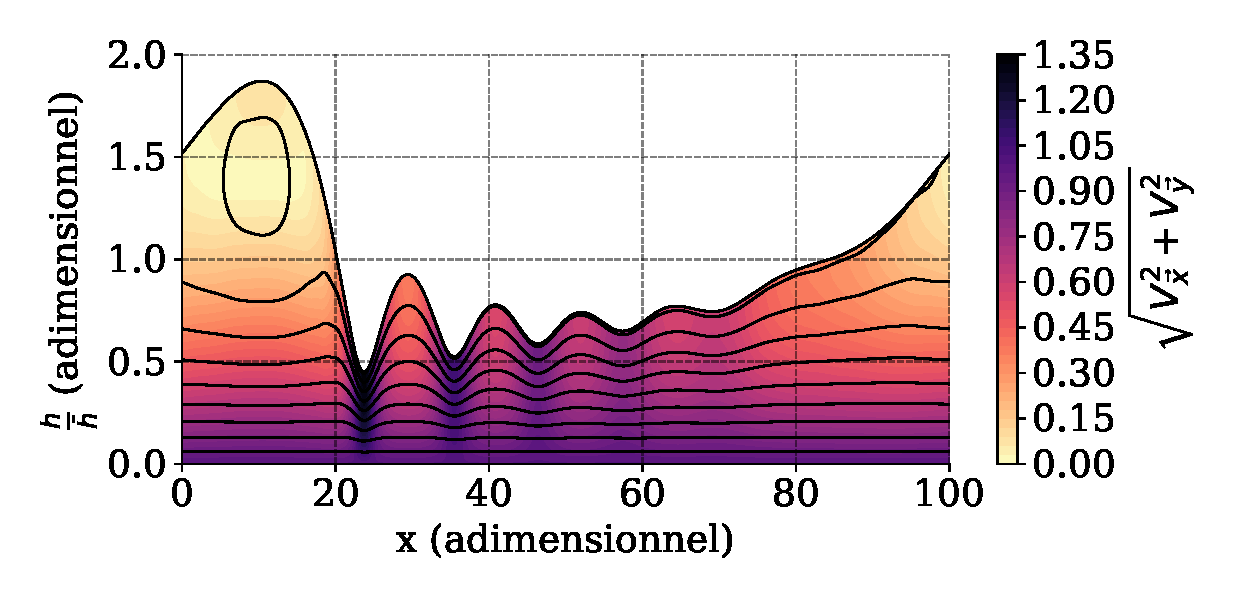
\includegraphics[width=0.95\columnwidth]{01-established_wave_streamlines}
            \captionof{figure}{Lignes de courants dune onde propagative, film vertical. ($\mathrm{Re}=20$, eau à 20 °C)}
            \label{fig:streamlines}
        \end{center}\vspace{.5cm}
    \end{multicols}

    On observe nettement les effets de recirculation au sein de l'onde décrits par \textcite{Brauner1989}, \textcite{Yoshimura1996} ou \textcite{Miyara1999}.

    \subsection*{Couplage thermique}
    Suivant un développement analogue, un modèle asymptotique a été écrit basé sur les équations de Fourrier (publication en cours d'écriture). Le profil de température est écrit comme une fonction de deux variables: $\theta = T|_{\bar{y}=0}$ et $\frac{\phi}{h} = \left.\partial_{y}T\right|_{\bar{y}=1}$, et l'intégration des résidus pondérés sur la hauteur du film mène à deux équations différentielles supplémentaire.

    \begin{multicols}{2}
        \begin{center}
            \includegraphics[width=0.98\columnwidth]{01-established_wave_T}
            \captionof{figure}{Champs de température ($\mathrm{Re}=20$, eau à 20°C)}
            \label{fig:thermal}
        \end{center}
        \columnbreak
        \begin{center}
            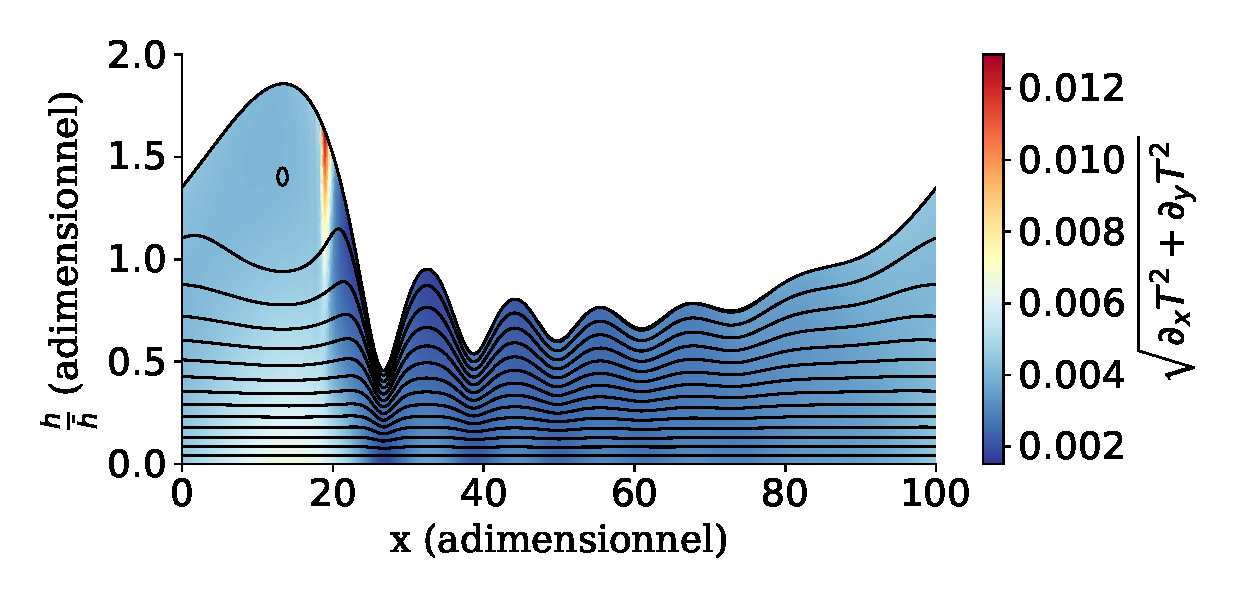
\includegraphics[width=0.98\columnwidth]{01-established_wave_Tmag_streamlines}
            \captionof{figure}{Magnitude du gradient de température et lignes de courant ($\mathrm{Re}=20$, $\mathrm{Bi} = 0.1$, eau à 20°C)}
            \label{fig:streamlines_thermal}
        \end{center}
    \end{multicols}

    On observe nettement un front thermique situé proche du point de stagnation du fluide au sein de la vague. A noter que le modèle n'est pas assez complexe pour représenter correctement ce phénomènes.

    \columnbreak

    \subsection*{Impact de la fréquence de forçage}

    \begin{multicols}{2}
        \subsubsection*{Sur l'hydrodynamique}

        \begin{center}
            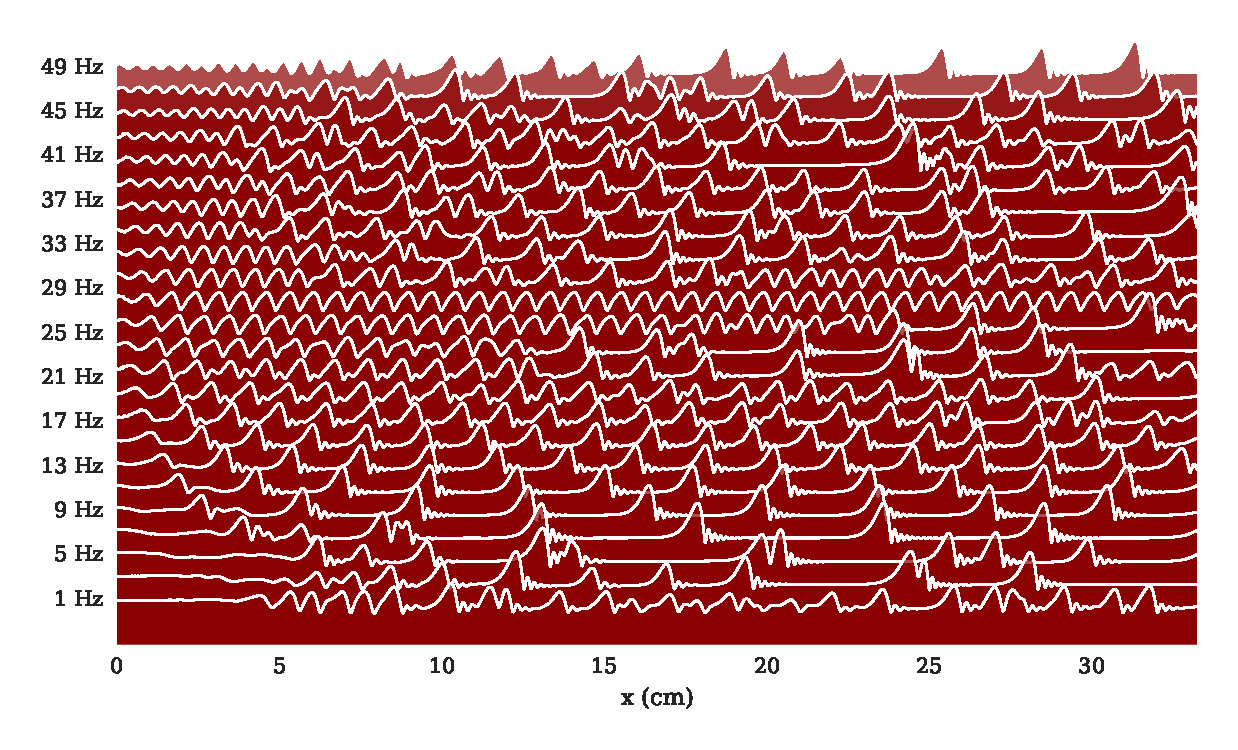
\includegraphics[width=0.98\columnwidth]{01-frequency_effect}
            \captionof{figure}{Plaque verticale avec forçage (3Hz à 18 Hz) bruité en entrée ($\mathrm{Re}=20$, eau à 20°C)}
            \label{fig:freq_effect}
        \end{center}

        Pour de haute et de basses fréquences, les ondes naturelles dominent. Entre les deux, des trains d'ondes saturés sont présents sur une grande partie de la plaque. Lorsque la fréquence est importante, les ondes capillaires ne sont plus observables.

        \columnbreak

        \subsubsection*{Sur l'intensification de transfert}
    \end{multicols}

    \section*{Suite des travaux}

    \begin{multicols}{2}
        \subsection*{Prise en compte de la turbulence}
        Les Reynolds présentés sont un Reynolds moyen, basé sur le film plat équivalent. Il peut être bien plus élevé, en particulier à la crête des ondes.

        L'objectif est de réécrire le modèle en incluant une viscosité turbulente via des lois de comportements usuelles. Les tourbillons de petites échelles sont pris en compte via leurs dissipations d'énergie au sein de l'écoulement.

        \columnbreak

        \subsection*{Effet Marangoni et \emph{dry patchs}}
        L'effet Marangoni est lié à la dépendance entre les caractéristique du fluide et la température (ou la concentration d'un solvant), en particulier sur la tension de surface.

        Cet effet mène à une instabilité supplémentaire, souvent dans le sens transverse de l'écoulement et mène à la formation de rivulets, et à un assèchement local de l'écoulement dans les cas extrêmes.

    \end{multicols}

\end{multicols}

\begin{center}
    \line(1,0){1500}
\end{center}

\begin{multicols}{2}
    \begin{center}
        \begin{tabular}{|c|c|}
            \hline $\rho$ & masse volumique \\
            \hline $u$ ou $V$ & champs de vitesse \\
            \hline $p$ & pression \\
            \hline $\tau$ & tenseur des contraintes \\
            \hline $h$ & hauteur de l'interface \\
            \hline
        \end{tabular}
        \begin{tabular}{|c|c|}
            \hline $q$ & débit local \\
            \hline $f$ & force volumique \\
            \hline $\mathrm{Ct}$ & Facteur de pente \\
            \hline $\mathrm{Re}$ & Nombre de Reynolds \\
            \hline $\mathrm{W\!e}$ & Nombre de Weber \\
            \hline $\mathrm{Bi}$ & Nombre de Biot \\
            \hline
        \end{tabular}
    \end{center}

        Encadrement de thèse :
        \begin{itemize}
            \item C. Ruyer - Quil (LOCIE)
            \item N. Caney (LEGI)
            \item P. Bandelier (CEA - Liten)
        \end{itemize}

        Partenaire industriel : CIAT

        Mis en place et soutenu par la région Rhône-Alpes
\end{multicols}

\end{document}
